% !TeX program = lualatex -synctex=1 -interaction=nonstopmode --shell-escape %.tex

\documentclass[12pt, table]{exam}
\usepackage[eng]{borochkin}

\usepackage{borochkin_exam_eng}

%%%%%%%%%%%%%%%%%%%%%%%%%%%%%%%%%%%%%%%%%

\professor
\iftagged{professor}{ \printanswers }

%%%%%%%%%%%%%%%%%%%%%%%%%%%%%%%%%%%%%%%%%

\begin{document}
\setcounter{section}{0\relax}%
\noindent
% Control № #1, Variant #2, Subject #3
\studentpersonalinfo{1}{1}{IF}
\normalsize

\begin{questions}
\question[40] Test
\answerstotestShort
	
\question[20] The table below shows how the USDRUB exchange rate fluctuated from 01.11.2014 to 01.11.2015. Option expiration date is 01.01.2016 (option term is 2 months). Option execution price is 75 roubles per 1 US dollar. The USD risk free rate is 1\% annual, the RUB risk free rate is 8\% annual. Use binomial option pricing model as a methodology. 

Evolution of USDRUB exchange rate during 01.11.2014 to 01.11.2015 period of time:
\begin{table}[htbp]
\centering
\begin{tabular}{rr}
	\toprule
	Date & Exchange rate \\ \midrule
	11/1/2014 &       49.3837 \\
	12/1/2014 &       60.2065 \\
	1/1/2015 &       69.6717 \\
	2/1/2015 &       61.7096 \\
	3/1/2015 &         58.09 \\
	4/1/2015 &       51.4724 \\
	5/1/2015 &       52.2844 \\
	6/1/2015 &       55.1546 \\
	7/1/2015 &       61.3668 \\
	8/1/2015 &       64.2563 \\
	9/1/2015 &       65.3079 \\
	10/1/2015 &       63.4648 \\
	11/1/2015 &        66.061
\end{tabular}%
\end{table}


\begin{subparts}
\subpart[5] Calculate mean and standard deviation of currency rate monthly returns
\begin{solution}[8em]
	
	m = 2.9080\%
	
	s = 10.1345\%	
\end{solution}

\subpart[10] Compute the call option price if the purchase is planned at 01.11.2015.
\begin{solution}[20em]
	
	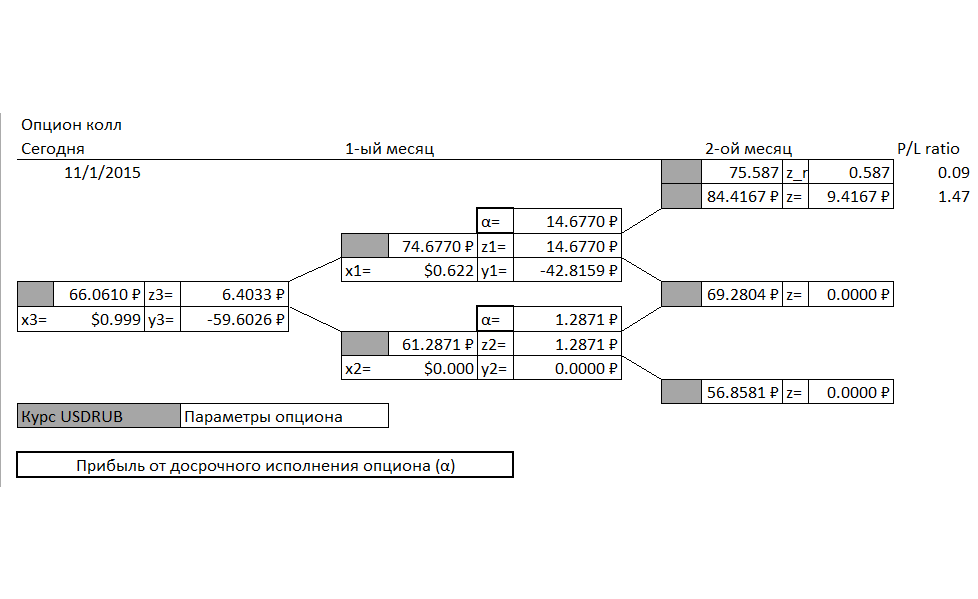
\includegraphics[height=8.5cm]{img/option_call_usdrub.png}
\end{solution}

\subpart[5] Suppose, the USDRUB exchange will reach 72,0633 at 01.12.2015 and 75,587 at 01.01.2016. How much profit would trader make if he invested 1000 USD in this financial instrument at 01.11.2015.
\begin{solution}[8em]

$$\frac{0.587~₽}{6.4033~₽} \cdot 100\% = 9\% $$

\end{solution}
	
\end{subparts}
\addpoints

\pagebreak
\question[10] The Russian enterprise attracts 50 000 US dollars as a loan under fixed rate of 15\% per annum for the period of 15 months. The USD/RUR exchange rate was 36,00 at the time of the credit deal with the bank. What has to be the value of a USD/RUR exchange rate at the time of loan repayment so that the financial resources ruble cost was zero?

\begin{solution}[8em]

Loan, USD	50000

Fixed interest rate, \%	20\%

Period, years	1,25

USD/RUR exchange rate	36

Loan plus interest, USD	62500

Demanded USD/RUR exchange rate	30,32

\end{solution}

\question[10] The enterprise prepares the project. For this purpose it needs to attract 3.5 million rubles for the term of 1 year 3 months. After the project end it will be able to return no more than 4,5 million rubles to the creditor. The enterprise has possibility to attract the loan in foreign currency. A current USD/RUR rate is 36,00. The loan must be repaid at the end of the period with interest. According to forecasts, in 1 year and 3 months USD/RUR rate will make from 37,00 to 40,00. What are the minimal and maximal acceptable interest rates of the loan?

\begin{solution}[8em]
	
	Loan, mln RUR	3,5
	
	Period, years	1,25
	
	Loan limit, mln RUR	4,5
	
	Current RUR/USD rate	36
	
	Maximal forecasted RUR/USD rate	37
	
	Minimal forecasted RUR/USD rate	40
	
	Loan, mln USD	0,0972
	
	Maximal loan, mln USD	0,12
	
	Minimal loan, mln USD	0,1125
	
\end{solution}
\end{questions}


\pagebreak
\noindent\textbf{Tests (choose one the most suitable answer)}

\begin{questions}
\begin{multicols}{2}
\setlength{\columnsep}{1cm}

\question During economic globalization a share of direct foreign investments in the total amount of world investments:
	 \begin{choices}
	 \CC grows;
	 \choice decreases;
	 \choice remains invariable;
	 \choice changes in an unpredictable way.
	 \end{choices}
\question During globalization the stability of developing countries financial markets:
	 \begin{choices}
	 \choice increases;
	 \CC decreases;
	 \choice remains invariable;
	 \choice changes in an unpredictable way.
	 \end{choices}
\question What does of the listed measures promote restriction of the international movement of the speculative capital:
	 \begin{choices}
	 \choice increase in regulation of the banks international financial operations;
	 \choice imposing a tax on foreign exchange operations;
	 \choice increase of national interest rates;
	 \CC all abovementioned.
	 \end{choices}
\question The international financial market open hours are:
	 \begin{choices}
	 \choice from 8 to 18 Coordinated Universal Time (UTC);
	 \choice from 6 to 20 UTC;
	 \choice from 4 to 22 UTC;
	 \CC round the clock.
	 \end{choices}
\question The greatest risk level characterizes operations of the following participants of the international financial market:
	 \begin{choices}
	 \CC speculators traders;
	 \choice arbitrageurs;
	 \choice intermediaries;
	 \choice hedgers.
	 \end{choices}
\question In the conditions of the global financial market local financial crises:
	 \begin{choices}
	 \choice are sharply weakened;
	 \choice don't undergo changes;
	 \CC develop into regional and world crises;
	 \choice anything from the listed.
	 \end{choices}
\question Democratization of the country promotes:
	 \begin{choices}
	 \CC strengthening of the national financial market integration into the world;
	 \choice weakening of the national financial market integration into the world;
	 \choice the invariable level of the national financial market integration into the world;
	 \choice unpredictable changes of the level of the national financial market integration into the world.
	 \end{choices}
\question In the modern international financial market the competition between participants:
	 \begin{choices}
	 \CC grows;
	 \choice decreases;
	 \choice remains at invariable level;
	 \choice changes without a certain tendency.
	 \end{choices}
\question Major factors of the world financial market development at present are:
	 \begin{choices}
	 \choice gold demonetization;
	 \CC integration of the national financial markets of developing countries into the international financial market;
	 \choice growth of the knowledge intensive branches of world economy;
	 \choice narrowing of a range of financial instruments.
	 \end{choices}
\question The currency market is most closely connected with:
	 \begin{choices}
	 \choice production;
	 \CC foreign trade;
	 \choice domestic trade;
	 \choice consumption.
	 \end{choices}
\question The largest participants of the currency market have more advantages in comparison with small and average participants on:
	 \begin{choices}
	 \choice open market;
	 \CC over-the-counter market;
	 \choice forward market;
	 \choice spot market.
	 \end{choices}
\question By abbreviation of OTS it is designated:
	 \begin{choices}
	 \choice open currency market;
	 \CC over-the-counter currency market;
	 \choice forward currency market;
	 \choice spot currency market.
	 \end{choices}
\question The exchange rate expresses:
	 \begin{choices}
	 \choice purchasing power of currency;
	 \choice usefulness of currency;
	 \CC proportion of an exchange of one currency to another;
	 \choice some social convention.
	 \end{choices}
\question Essential divergences of official and market currency exchange rate are characteristic for:
	 \begin{choices}
	 \choice the countries with exportoriented economy;
	 \choice the countries with the economy focused on selfsufficiency;
	 \CC the countries with state planning economy;
	 \choice the countries with free market economy.
	 \end{choices}
\question For forecasting of currency exchange rates in longterm is more effective:
	 \begin{choices}
	 \choice technical analysis;
	 \CC fundamental analysis;
	 \choice graphic analysis;
	 \choice all three methods are equally effective.
	 \end{choices}
\question Growing inflationary expectations in Russia would lead a ruble exchange rate versus world currencies:
	 \begin{choices}
	 \choice increase;
	 \CC decrease;
	 \choice invariable;
	 \choice change in an unpredictable way.
	 \end{choices}
\question Longterm decrease in a national currency exchange rate will have the following impact on the structure of national economy:
	 \begin{choices}
	 \CC growth of exports, decrease of imports;
	 \choice decrease exports, growth imports;
	 \choice lack of changes;
	 \choice unpredictable changes.
	 \end{choices}
\question To increase national currency convertibility the national government should:
	 \begin{choices}
	 \choice increase exchange rate of the national currency;
	 \CC cancel restrictions on currency operations;
	 \choice refuse to regulate currency exchange rate;
	 \choice issue national currency.
	 \end{choices}
\question USD/RUR makes 36,00 EUR/RUR makes 48,60 USD/RUR makes:
	 \begin{choices}
	 \CC 1 dollars = 0,74 euros;
	 \choice 1 dollars = 0,35 euros;
	 \choice 1 dollars = 1,20 euros;
	 \choice 1 dollars = 1,35 euros.
	 \end{choices}
\question The spread on less stable currency is equal A, the spread on stable currency is equal B In this case:
	 \begin{choices}
	 \CC A is more than B;
	 \choice A is less than B;
	 \choice A slightly differs from B;
	 \choice A differs in an unpredictable way from B.
	 \end{choices}



\end{multicols}
\end{questions}

\end{document}
